
%(BEGIN_QUESTION)
% Copyright 2012, Tony R. Kuphaldt, released under the Creative Commons Attribution License (v 1.0)
% This means you may do almost anything with this work of mine, so long as you give me proper credit

Identifiser hensikten med forholdsregulatoren for flow FFC-41 i denne destillasjonsprosessen:

$$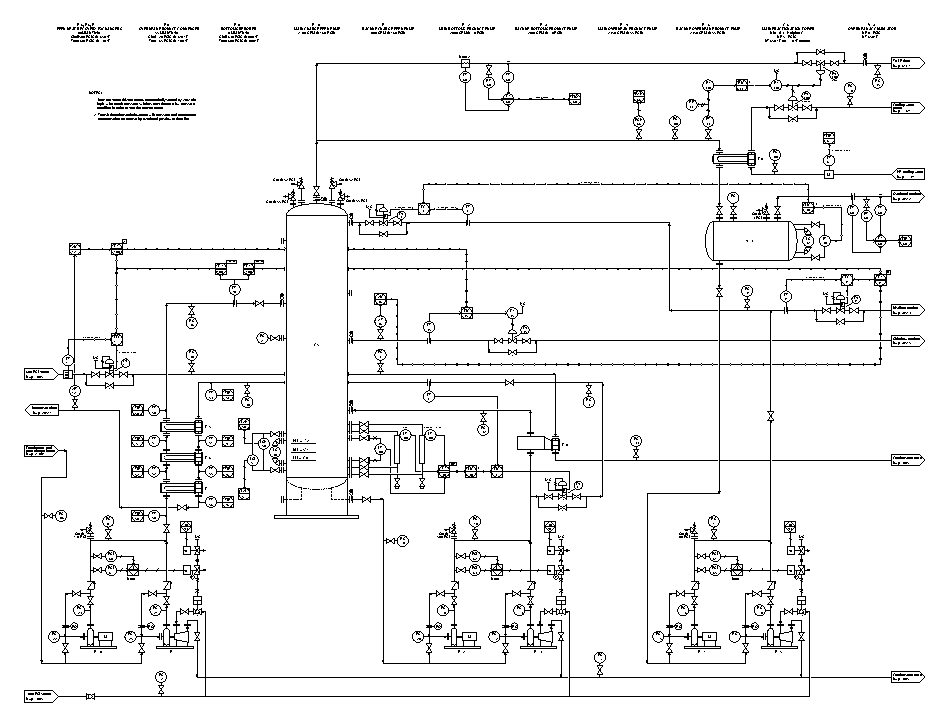
\includegraphics[width=15.5cm]{i0001rx01.eps}$$



\underbar{file i01262}
%(END_QUESTION)





%(BEGIN_ANSWER)

Hensikten med FFC-41 er å styre dampstrømmen på 600 PSI til bunnreboileren (varmeveksler E-9) i forhold til innkommende mateflow. Mateflowen er derfor den «frie» flowen, mens dampflowen er den «bundne» flowen. Forholdet mellom dampflow og mateflow justeres automatisk av AIT-42, som måler noe ved sammensetningen i bunnproduktet (kanskje tetthet, kokepunkt eller en annen egenskap relatert til destillasjonen av produktene i kolonnen).
 
%(END_ANSWER)





%(BEGIN_NOTES)

\vskip 20pt \vbox{\hrule \hbox{\strut \vrule{} {\bf Virtuell feilsøking} \vrule} \hrule}

Dette spørsmålet egner seg godt som en «Virtuell feilsøking»-øvelse. Når du viser diagrammet til studentene, ser du først for deg en bestemt feil i systemet. Deretter presenterer du ett eller flere symptomer på denne feilen (noe en operatør eller annen bruker av systemet kan observere). Studentene foreslår så ulike diagnostiske tester som kan utføres på systemet for å identifisere feilens art og plassering, som om de var teknikere som feilsøker problemet. Din oppgave er å fortelle hva resultatet(-ene) ville blitt for hver foreslåtte test, og dokumentere disse resultatene slik at alle studentene kan se dem.

Under og etter øvelsen er det nyttig å stille oppfølgingsspørsmål som:

\begin{itemize}
\item{} Hva forteller resultatet av den siste diagnostiske testen om feilen?
\item{} Anta at resultatet av den siste diagnostiske testen var annerledes. Hva ville det resultatet da fortelle om feilen?
\item{} Er den siste diagnostiske testen den beste vi kunne gjort?
\item{} Hva ville vært den ideelle rekkefølgen på tester for å diagnostisere problemet med færrest mulig steg?
\end{itemize}


%INDEX% Process: distillation, generic (realistic P\P&IDID shown)

%(END_NOTES)

